\documentclass[aip,amsmath, reprint, author-year]{revtex4-1}
\usepackage{url}

\usepackage{hyperref}
\usepackage{graphicx} % for graphics
%\usepackage{listings} % for code listtings
%\usepackage{color}

%\setcitestyle{round, author-year}

\setcounter{page}{1}

%\bibliographystyle{aipauth4-1.bst}

\begin{document}

\begin{abstract}
Using Generalised Process Capability Data to Reduces: Rework, Cost, Failure Rate, Assembly Problems and Increases Product Performance by using process capability from previous products.
A description of the concept of generalisation, uses and implementation strategy.
\end{abstract}

\title{Use of General Process Capability Data}
\author{Andreas Bruun Okholm, s082562\\
Mathias Rask Møller, s082536 }
\affiliation{Technical University of Denmark}
 
\date{\today}
\maketitle

%Introduction

\section{Introduction}

robust design general

\section{Statistics}

a measurement
a measurement set
std and bias
cpk 
\begin{equation}
C_{pk} = \frac{bias}{3 \, \sigma}
\label{eq:sddj}
\end{equation}


confidence intevals

\section{How much data}


\begin{figure}
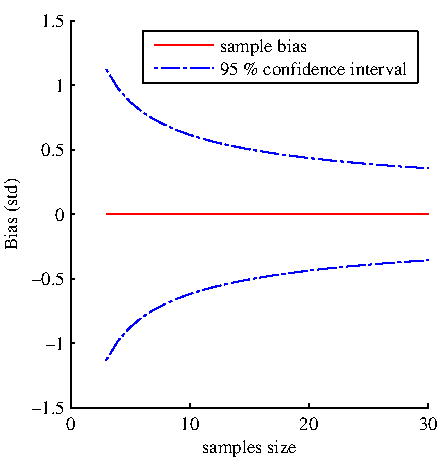
\includegraphics{stats_bias_confidence.pdf}
\caption{\label{fig:std_uncertainty}The uncertainty of the standard deviation estimate is reduced as the number of samples is increased. The increase in accuracy gained per additional decreases with more samples. From the graph we have chosen 12 to be the optimal point for general process capability use.}
\end{figure}



\begin{figure}
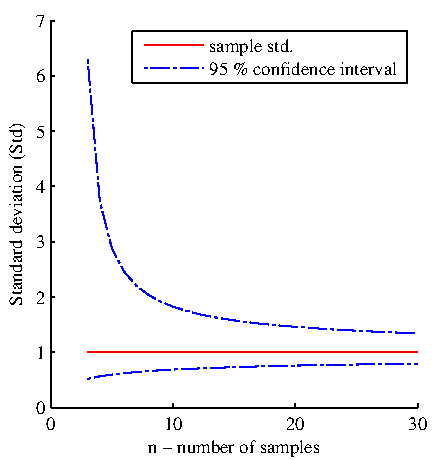
\includegraphics{stats_std_confidence.pdf}
\caption{\label{fig:std_uncertainty}The uncertainty of the standard deviation estimate is reduced as the number of samples is increased. The increase in accuracy gained per additional decreases with more samples. From the graph we have chosen 12 to be the optimal point for general process capability use.}
\end{figure}




sample size  \ref{eq:sddj}




Obtaining Process Capability data is a process of measuring a lot of products.
Products are measured and compared to the nominal size they were produced for, this is called error.

In a production line control measurement are usually done by taking a set of samples to represent the entire population. Each product in the sample set, produces a measurement. From the set of measurements a standard deviation and a mean shift is calculated.

\section{uses}
existance of it-grade
improvement per rework
material selection



In the design process is often a problem to apply tolerances. This aspect of the design phase is often pushed to the very end before production. Features are designed so delicate that in order to meet specification tight tolerances are applied, which can be difficult to produce.
This problem could be solved by looking up the critical tolerance the industry typically can produce to and altering the design for a suitable tolerance.  I that way making tolerance selection a part of the design process.

By looking at normalized data of the variance of products of the same material and process, it is possible to find a suitable tolerance

\section{implementation}




Industry secrets
	experience
	
	
active actors and interest groups
	sub suppliers 
	mechanical design consultants
	

difficulties
	Non disclusure agreement
	end-customer
	

\section*{References}
\bibliography{../PCDBmasterBibliography/PCDB_Master_bib.bib}

\end{document}